\chapter{Project Planning Methodology}

Given the limited amount of time and the scope of this project, having working prototypes in short periods of time enables us to test and change our design decisions in case the obtained results do not cope with our expected goals.  

Agile is an iterative and incremental software development methodology which focuses on flexibility, interactivity, and a high level of transparency. Each agile iteration, known as sprint, has a detailed feature list that the developer aims to have implemented and tested by the end of that sprint.

Considering that we are building a platform, having users perspective on mind is essential through all the development process. In Agile, user stories are an excellent way to achieve that by defining features as what a specific type of user wants to do with the system and why. 

Furthermore, user stories allows us to easily develop quality assurance tests that validate use cases and scenarios rather than validating just functions implementations. This is known as \textit{Persona Based Testing}, where a a fictional user profile is created to represent a user type with specific characteristics that expects certain high-level functionalities to be provided by the product being developed.

We will use GitHub \cite{github} to keep track of all changes made through the entire development of the project, and along with the ZenHub \cite{zenhub} plugin, we will use it as our project planning tool. This plugin adds several features in order to integrate Agile development into Github. 

A list of the most important features from GitHub and ZenHub that we will use in our project planning are described below.

\paragraph*{Issues.} Despite its name, apart from reporting bugs, they can be used to track enhancements ideas, features requests or tasks. As seen in Figure \ref{fig:issue}, we will use issues mainly to create and keep track of features requests as user stories. 

\begin{figure}[h!]
		\centering
    	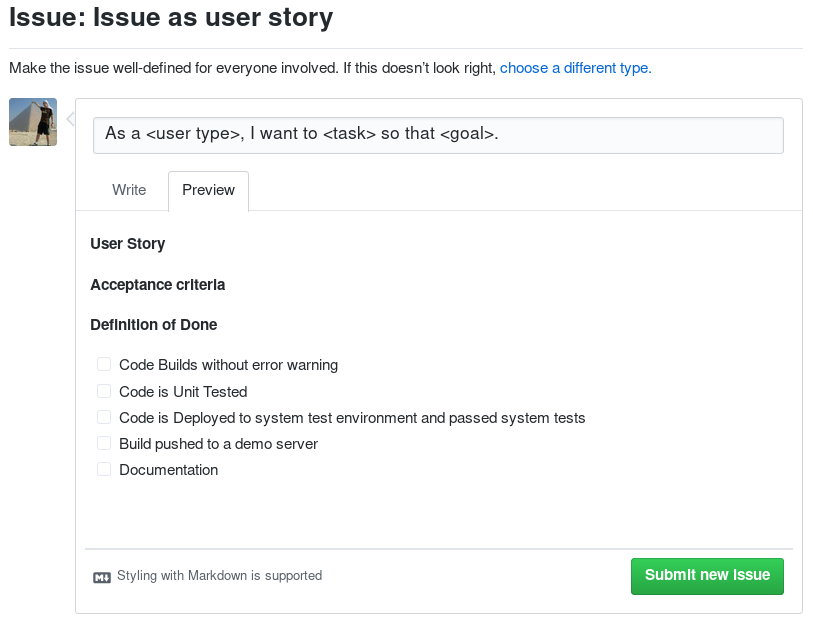
\includegraphics[width=\linewidth]{assets/images/issue-structure.png}
    	\caption{Structure of a user story asking for a new feature.}
    	\label{fig:issue}
\end{figure}

\paragraph*{Epics.} In Agile, it is the biggest unit of work. Essentially, it is a set of related user-stories that act as a big story together. For example, if "As an examiner I want to know the context of the problem so that I can better understand the topics involved in this project", then, the entire documentation process can be an Epic.

\begin{figure}[h!]
		\centering
    	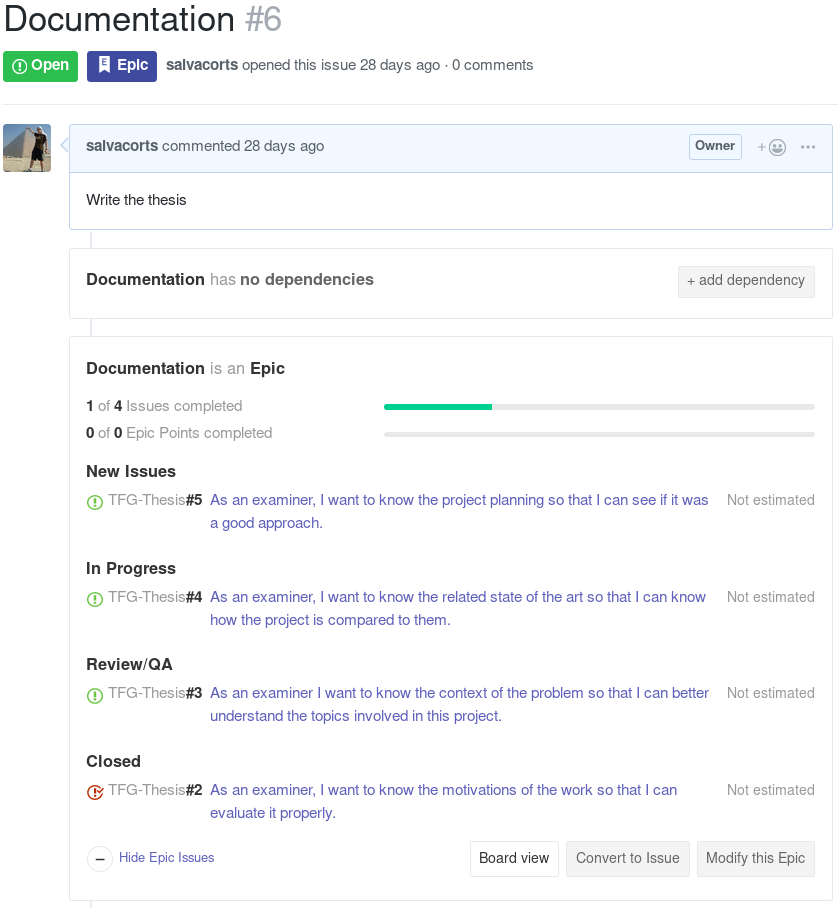
\includegraphics[width=\linewidth]{assets/images/epic.png}
    	\caption{Example of an Epic about this document.}
    	\label{fig:epic}
\end{figure}

\paragraph*{Milestones.} Are the GitHub equivalent to Agile sprints A given set of issues can be included on a milestone and by the end of the sprint these issues should have been solved. Once a sprint starts its content should remain unchanged until the deadline is reached.

\paragraph*{Project Board.} In order to have an overview of the current project development state, ZenHub provides a Kanban board \cite{kanban} where issues can be divided into categories and sorted by difficulty or priority among other options. We will divide our issues into three categories according to their current stage on the development process:

\begin{enumerate}
	\item \textbf{New Issues:} Features that we have not started working on yet nor are not in the \textit{Icebox}.
	
	\item \textbf{Icebox:} Issues that fall into this category are nice to have features that have low-priority and therefore will not be implemented unless time is left or their priority increases.  
	
	\item \textbf{In Progress:} Features that we are implementing at the moment.
	
	\item \textbf{Review/QA:} Features that have been already implemented and are waiting to be reviewed for approval or tested.
	
	\item \textbf{Closed:} Features that are part of the final product to be delivered and have passed all tests and reviews successfully.
\end{enumerate}

\begin{figure}[h!]
		\centering
    	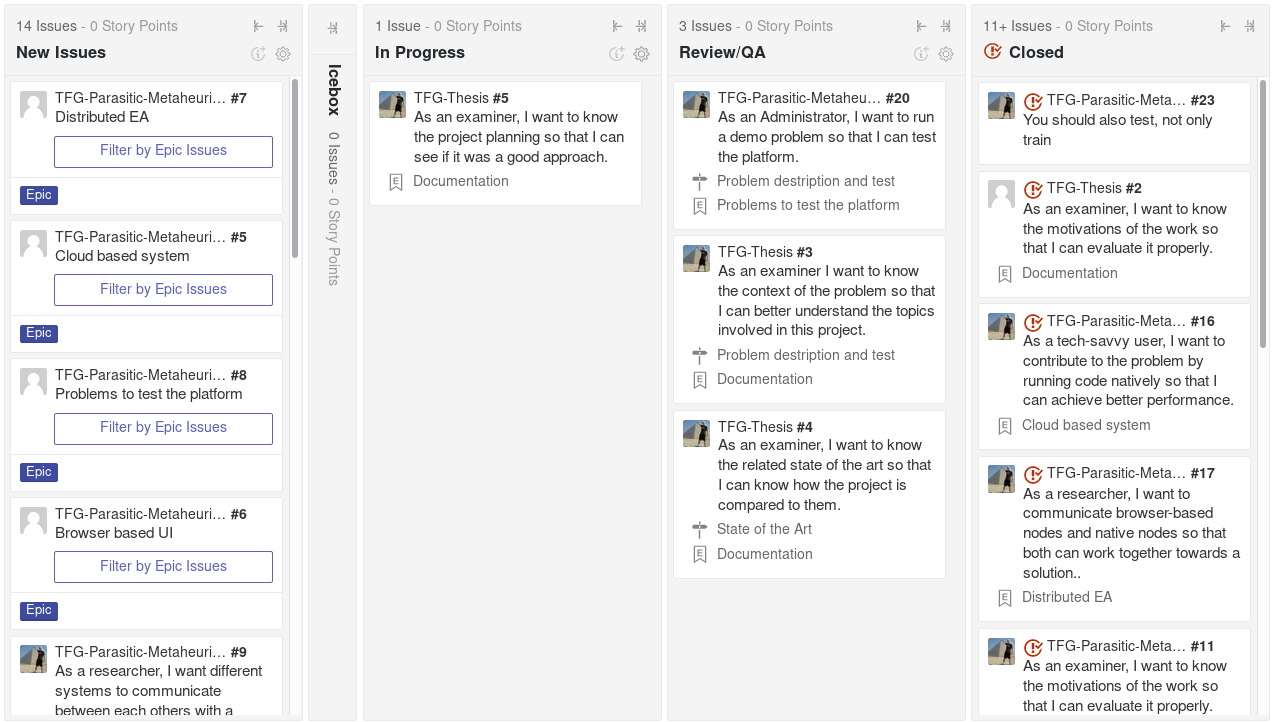
\includegraphics[width=\linewidth]{assets/images/board.png}
    	\caption{Project board.}
    	\label{fig:board}
\end{figure}


\section{Personas}
As previously stated, it is indispensable for a platform to be tested from its users perspective; so that, \textit{Persona Based Testing} will be the quality assurance methodology to be followed. We have created the following personas to create our GitHub issues and tests.

\paragraph*{Antonio}

\paragraph*{Blanca}

\paragraph*{Luis}

\paragraph*{Ana}
  